\documentclass{beamer}

\usepackage{beamerthemeCambridgeUS}
\usepackage{textpos}
\usepackage{ragged2e}
\usepackage{ulem}

\graphicspath{{G:/My Drive/FIGURAS/}}

\title[Cartografía Geomorfológica]{GEOMORFOLOGÍA}
\author[Edier Aristizabal]{Edier V. Aristizábal G.}
\institute{evaristizabalg@unal.edu.co}
\date{\tiny{Versión:\today}}

\addtobeamertemplate{headline}{}{%
	\begin{textblock*}{2mm}(.9\textwidth,0cm)
	\hfill\includegraphics[height=1cm]{un}  
	\end{textblock*}}

\begin{document}
%%%%%%%%%%%%%%%%%%%%%%%%%%%%%%%%%%%%%%%%%%%%%%%%%%%%%%%%%%%%%%%%%%%%%%%%%
\begin{frame}
\titlepage
\centering
   	\includegraphics[width=2cm]{unal} 
\end{frame}
%%%%%%%%%%%%%%%%%%%%%%%%%%%%%%%%%%%%%%%%%%%%%%%%%%%%%%%%%%%%%%%%%%%%%%%%%
\begin{frame}
\frametitle{Definición}
\small{Es el conjunto de estudios y operaciones \textbf{científicas, artísticas y técnicas} que intervienen, a partir de los resultados de las observaciones directas o de la explotación de una documentación, en el establecimiento de mapas, planos y otras formas de expresión, así como en su utilización. (Joly, 1979) }

\begin{center}
   	\includegraphics[scale=0.28]{Geomorphological-map}
\end{center}
\end{frame}
%%%%%%%%%%%%%%%%%%%%%%%%%%%%%%%%%%%%%%%%%%%%%%%%%%%%%%%%%%%%%%%%%%%%%%%%%
\begin{frame}
\frametitle{Cartografía básica $\rightarrow$ Cartografía temática}
\begin{center}
   	\includegraphics[scale=0.48]{cartobasica}
\end{center}
\end{frame}
%%%%%%%%%%%%%%%%%%%%%%%%%%%%%%%%%%%%%%%%%%%%%%%%%%%%%%%%%%%%%%%%%%%%%%%%%
\begin{frame}
\frametitle{Elementos de la cartografía básica}
\begin{center}
   	\includegraphics[scale=0.40]{punto}
\end{center}
\end{frame}
%%%%%%%%%%%%%%%%%%%%%%%%%%%%%%%%%%%%%%%%%%%%%%%%%%%%%%%%%%%%%%%%%%%%%%%%%
\begin{frame}
\frametitle{Elementos de la cartografía básica}
\begin{center}
   	\includegraphics[scale=0.42]{fueraescala}
\end{center}
\end{frame}
%%%%%%%%%%%%%%%%%%%%%%%%%%%%%%%%%%%%%%%%%%%%%%%%%%%%%%%%%%%%%%%%%%%%%%%%%
\begin{frame}
\frametitle{Elementos de la cartografía básica}
\begin{center}
   	\includegraphics[scale=0.5]{elementsolineales}
\end{center}
\end{frame}
%%%%%%%%%%%%%%%%%%%%%%%%%%%%%%%%%%%%%%%%%%%%%%%%%%%%%%%%%%%%%%%%%%%%%%%%%
\begin{frame}
\frametitle{Elementos de la cartografía básica}
\begin{center}
   	\includegraphics[scale=0.5]{elementosarea}
\end{center}
\end{frame}
%%%%%%%%%%%%%%%%%%%%%%%%%%%%%%%%%%%%%%%%%%%%%%%%%%%%%%%%%%%%%%%%%%%%%%%%%
\begin{frame}
\frametitle{Coordenadas Geográficas}
\begin{center}
   	\includegraphics[scale=0.5]{esferoide}
\end{center}
\end{frame}
%%%%%%%%%%%%%%%%%%%%%%%%%%%%%%%%%%%%%%%%%%%%%%%%%%%%%%%%%%%%%%%%%%%%%%%%%
\begin{frame}
\frametitle{GEOIDE}
\begin{center}
   	\includegraphics[scale=0.5]{geoide3}
\end{center}
\end{frame}
%%%%%%%%%%%%%%%%%%%%%%%%%%%%%%%%%%%%%%%%%%%%%%%%%%%%%%%%%%%%%%%%%%%%%%%%%
\begin{frame}
\frametitle{Proyección a coordenadas planas}
\small{\emph{You can’t represent Earth’s surface in two dimensions without distortion.}}
\begin{center}
   	\includegraphics[scale=0.55]{projec}
\end{center}
\end{frame}
%%%%%%%%%%%%%%%%%%%%%%%%%%%%%%%%%%%%%%%%%%%%%%%%%%%%%%%%%%%%%%%%%%%%%%%%%
\begin{frame}
\frametitle{Familias de proyección}
\begin{center}
   	\includegraphics[scale=0.45]{proye}
\end{center}
\end{frame}
%%%%%%%%%%%%%%%%%%%%%%%%%%%%%%%%%%%%%%%%%%%%%%%%%%%%%%%%%%%%%%%%%%%%%%%%%
\begin{frame}
\frametitle{Escala}
\begin{center}
   	\includegraphics[scale=0.40]{escala}
\end{center}
\end{frame}
%%%%%%%%%%%%%%%%%%%%%%%%%%%%%%%%%%%%%%%%%%%%%%%%%%%%%%%%%%%%%%%%%%%%%%%%%
\begin{frame}
\frametitle{Escala}
\small{La \textbf{escala numérica} se expresa mediante una fracción que indica la relación entre la distancia medida entre dos puntos en el mapa (numerador) y la correspondiente en el terreno (denominador) de modo directo entre unidades del sistema.}\\
\begin{center}
1:25.000
1:500
1:30.000
\end{center}
\small{La \textbf{escala gráfica} es una línea subdividida en segmentos para indicar longitudes sobre el mapa de las unidades terrestres de distancia}
\begin{center}
   	\includegraphics[scale=0.40]{escala4}
\end{center}
\end{frame}
%%%%%%%%%%%%%%%%%%%%%%%%%%%%%%%%%%%%%%%%%%%%%%%%%%%%%%%%%%%%%%%%%%%%%%%%%
\begin{frame}
\frametitle{Escala}
\begin{center}
   	\includegraphics[scale=0.35]{escala2}
\end{center}
\end{frame}
%%%%%%%%%%%%%%%%%%%%%%%%%%%%%%%%%%%%%%%%%%%%%%%%%%%%%%%%%%%%%%%%%%%%%%%%%
\begin{frame}
\frametitle{Resolución Espacial}
 \begin{figure}
    \centering
    \includegraphics[height=.7\textheight]{G:/My Drive/CATEDRA/ANALISIS GEOESPACIAL/fig/resolucion}
  \end{figure}
\end{frame}
%%%%%%%%%%%%%%%%%%%%%%%%%%%%%%%%%%%%%%%%%%%%%%%%%%%%%%%%%%%%%%
%%%%%%%%%%%%%%%%%%%%%%%%%%%%%%%%%%%%%%%%%%%%%%%%%%%%%%%%%%%%%%
\begin{frame}
\frametitle{Resolución Espacial}
 \begin{figure}
    \centering
    \includegraphics[height=.7\textheight]{G:/My Drive/CATEDRA/ANALISIS GEOESPACIAL/fig/pixel2}
  \end{figure}
\end{frame}
%%%%%%%%%%%%%%%%%%%%%%%%%%%%%%%%%%%%%%%%%%%%%%%%%%%%%%%%%%%%%%
\begin{frame}
 \begin{figure}
    \centering
    \includegraphics[height=.8\textheight]{G:/My Drive/CATEDRA/ANALISIS GEOESPACIAL/fig/pixel3}
  \end{figure}
\end{frame}
%%%%%%%%%%%%%%%%%%%%%%%%%%%%%%%%%%%%%%%%%%%%%%%%%%%%%%%%%%%%%%
\begin{frame}
\begin{exampleblock}{Rs vs. Px vs. GSD}
\small{La Rs es diferente al Px y al GSD. Sólo son iguales cuando se encuentra a resolución completa.}
\end{exampleblock}
 \begin{figure}
    \centering
    \includegraphics[height=.7\textheight]{G:/My Drive/CATEDRA/ANALISIS GEOESPACIAL/fig/hd}
  \end{figure}
\tiny{https://crisp.nus.edu.sg/~research/tutorial/rsmain.htm}
\end{frame}
%%%%%%%%%%%%%%%%%%%%%%%%%%%%%%%%%%%%%%%%%%%%%%%%%%%%%%%%%%%%%%
\begin{frame}
\frametitle{Resolución espacial vs. Escala}
 \begin{figure}
    \centering
    \includegraphics[height=.4\textheight]{G:/My Drive/CATEDRA/ANALISIS GEOESPACIAL/fig/escalavsres}
  \end{figure}
\end{frame}
%%%%%%%%%%%%%%%%%%%%%%%%%%%%%%%%%%%%%%%%%%%%%%%%%%%%%%%%%%%%%%
\begin{frame}
\frametitle{Área Mínima Cartografiable}
\framesubtitle{Criterio Salitchev (1979) 4mm x 4mm}
 \begin{figure}
    \centering
    \includegraphics[height=.8\textheight]{G:/My Drive/CATEDRA/ANALISIS GEOESPACIAL/fig/salitechv}
  \end{figure}
\end{frame}
%%%%%%%%%%%%%%%%%%%%%%%%%%%%%%%%%%%%%%%%%%%%%%%%%%%%%%%%%%%%%%
\begin{frame}
\frametitle{Tamaño del pixel adecuado}
 \begin{figure}
    \centering
    \includegraphics[height=.7\textheight]{G:/My Drive/CATEDRA/ANALISIS GEOESPACIAL/fig/UMC}
  \end{figure}
\end{frame}
%%%%%%%%%%%%%%%%%%%%%%%%%%%%%%%%%%%%%%%%%%%%%%%%%%%%%%%%%%%%%%
\begin{frame}
\frametitle{Tamaño del pixel adecuado}
\begin{exampleblock}{Regla de Waldo Tobler (1967) }
\small{\emph{"The rule is: divide the denominator of the map scale by 1,000 to get the detectable size in meters. The resolution is one half of this amount."\\
Map Scale = Raster resolution (in meters) * 2 * 1000}}
\end{exampleblock}
 \begin{figure}
    \centering
    \includegraphics[height=.4\textheight]{G:/My Drive/CATEDRA/ANALISIS GEOESPACIAL/fig/detectablesize}
  \end{figure}
\end{frame}
%%%%%%%%%%%%%%%%%%%%%%%%%%%%%%%%%%%%%%%%%%%%%%%%%%%%%%%%%%%%%%
\begin{frame}
\frametitle{Distribución de planchas 1:500.000}
\begin{center}
   	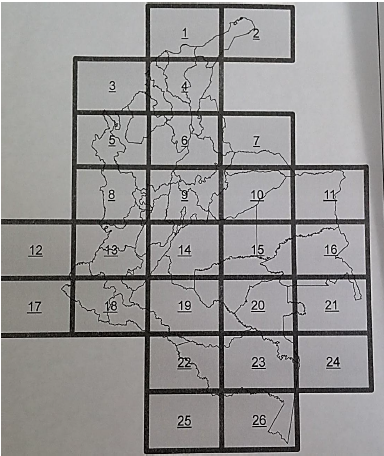
\includegraphics[scale=0.5]{planchas500k}
\end{center}
\end{frame}
%%%%%%%%%%%%%%%%%%%%%%%%%%%%%%%%%%%%%%%%%%%%%%%%%%%%%%%%%%%%%%%%%%%%%%%%%
\begin{frame}
\frametitle{Distribución de planchas 1:100.000}
\small{Una plancha 1:500.000 está dividida en 36 hojas escala 1:100.000 (100 miles) codificado en números.}
\begin{center}
   	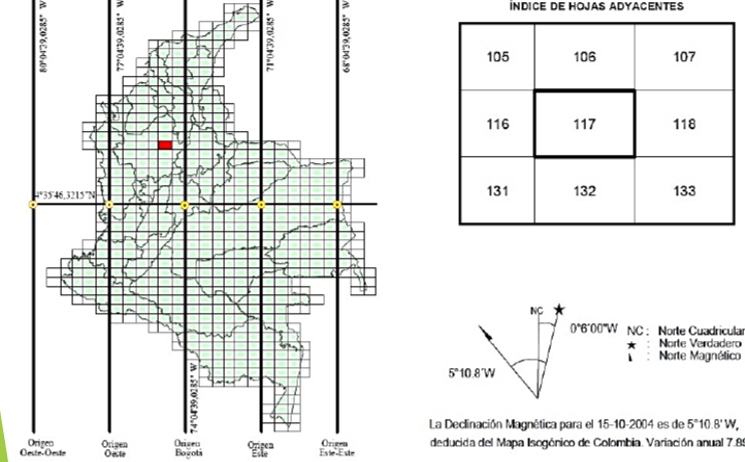
\includegraphics[scale=0.45]{planchas100k}
\end{center}
\end{frame}
%%%%%%%%%%%%%%%%%%%%%%%%%%%%%%%%%%%%%%%%%%%%%%%%%%%%%%%%%%%%%%%%%%%%%%%%%
\begin{frame}
\frametitle{Distribución de planchas 1:50.000}
\small{Una plancha 1:100.000 está dividida en 4 hojas escala 1:50.000 (50 miles) codificado en números romanos (I, II, III, IV).}
\begin{center}
   	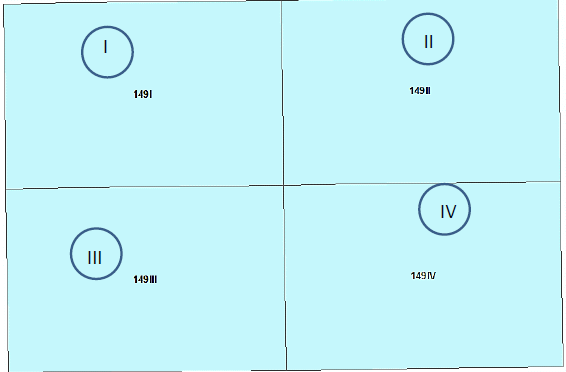
\includegraphics[scale=0.45]{planchas50k}
\end{center}
\end{frame}
%%%%%%%%%%%%%%%%%%%%%%%%%%%%%%%%%%%%%%%%%%%%%%%%%%%%%%%%%%%%%%%%%%%%%%%%%
\begin{frame}
\frametitle{Distribución de planchas 1:25.000}
\small{Una plancha 1:50.000 está dividida en 4 hojas escala 1:25.000 (50 miles) codificado en números romanos (A, B, C, D).}
\begin{center}
   	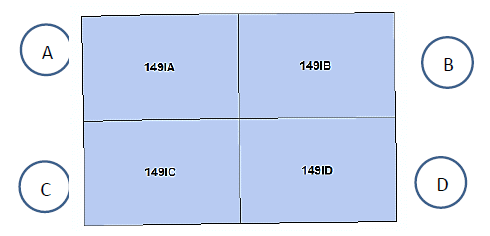
\includegraphics[scale=0.7]{planchas25k}
\end{center}
\end{frame}
%%%%%%%%%%%%%%%%%%%%%%%%%%%%%%%%%%%%%%%%%%%%%%%%%%%%%%%%%%%%%%%%%%%%%%%%%
\begin{frame}
\frametitle{Distribución de planchas 1:10.000}
\small{Una plancha 1:25.000 está dividida en 4 hojas escala 1:10.000 (50 miles) codificado en números romanos (1, 2, 3, 4).}
\begin{center}
   	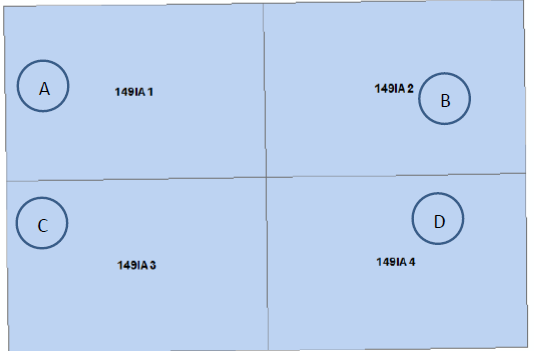
\includegraphics[scale=0.6]{planchas10k}
\end{center}
\end{frame}
%%%%%%%%%%%%%%%%%%%%%%%%%%%%%%%%%%%%%%%%%%%%%%%%%%%%%%%%%%%%%%%%%%%%%%%%%
\begin{frame}
\frametitle{Distribución de planchas 1:10.000}
\small{Una plancha 1:10.000 está dividida en 25 hojas escala 1:2.000 (50 miles) codificado en números romanos (a, b, c...,y).}
\begin{center}
   	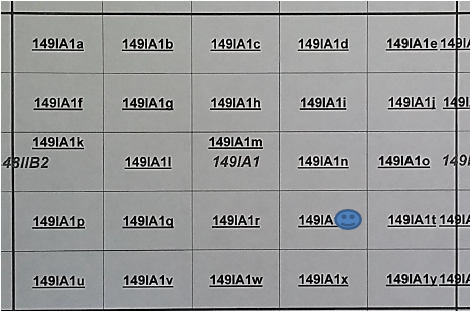
\includegraphics[scale=0.7]{planchas2k}
\end{center}
\end{frame}
%%%%%%%%%%%%%%%%%%%%%%%%%%%%%%%%%%%%%%%%%%%%%%%%%%%%%%%%%%%%%%%%%%%%%%%%%
\begin{frame}
\frametitle{IGAC}
\begin{center}
   	\includegraphics[scale=0.52]{geoportaligac}
   	\url{http://www.igac.gov.co/geoportal}
\end{center}
\end{frame}
%%%%%%%%%%%%%%%%%%%%%%%%%%%%%%%%%%%%%%%%%%%%%%%%%%%%%%%%%%%%%%%%%%%%%%%%%
\begin{frame}
\frametitle{Mapas temáticos -Geológico-}
\begin{center}
   	\includegraphics[scale=0.48]{mapageomorfologico}
\end{center}
\end{frame}
%%%%%%%%%%%%%%%%%%%%%%%%%%%%%%%%%%%%%%%%%%%%%%%%%%%%%%%%%%%%%%%%%%%%%%%%%
\begin{frame}
\frametitle{Mapas temáticos - Geomorfológico-}
\begin{center}
   	\includegraphics[scale=0.48]{mapageomorfologico1}
\end{center}
\end{frame}
%%%%%%%%%%%%%%%%%%%%%%%%%%%%%%%%%%%%%%%%%%%%%%%%%%%%%%%%%%%%%%%%%%%%%%%%%
\begin{frame}
\frametitle{Mapas temáticos - Geomorfológico-}
\begin{center}
   	\includegraphics[scale=0.4]{mapageomorfologico2}
\end{center}
\end{frame}
%%%%%%%%%%%%%%%%%%%%%%%%%%%%%%%%%%%%%%%%%%%%%%%%%%%%%%%%%%%%%%%%%%%%%%%%%
\begin{frame}
\frametitle{Metodologia ITC}
\begin{center}
   	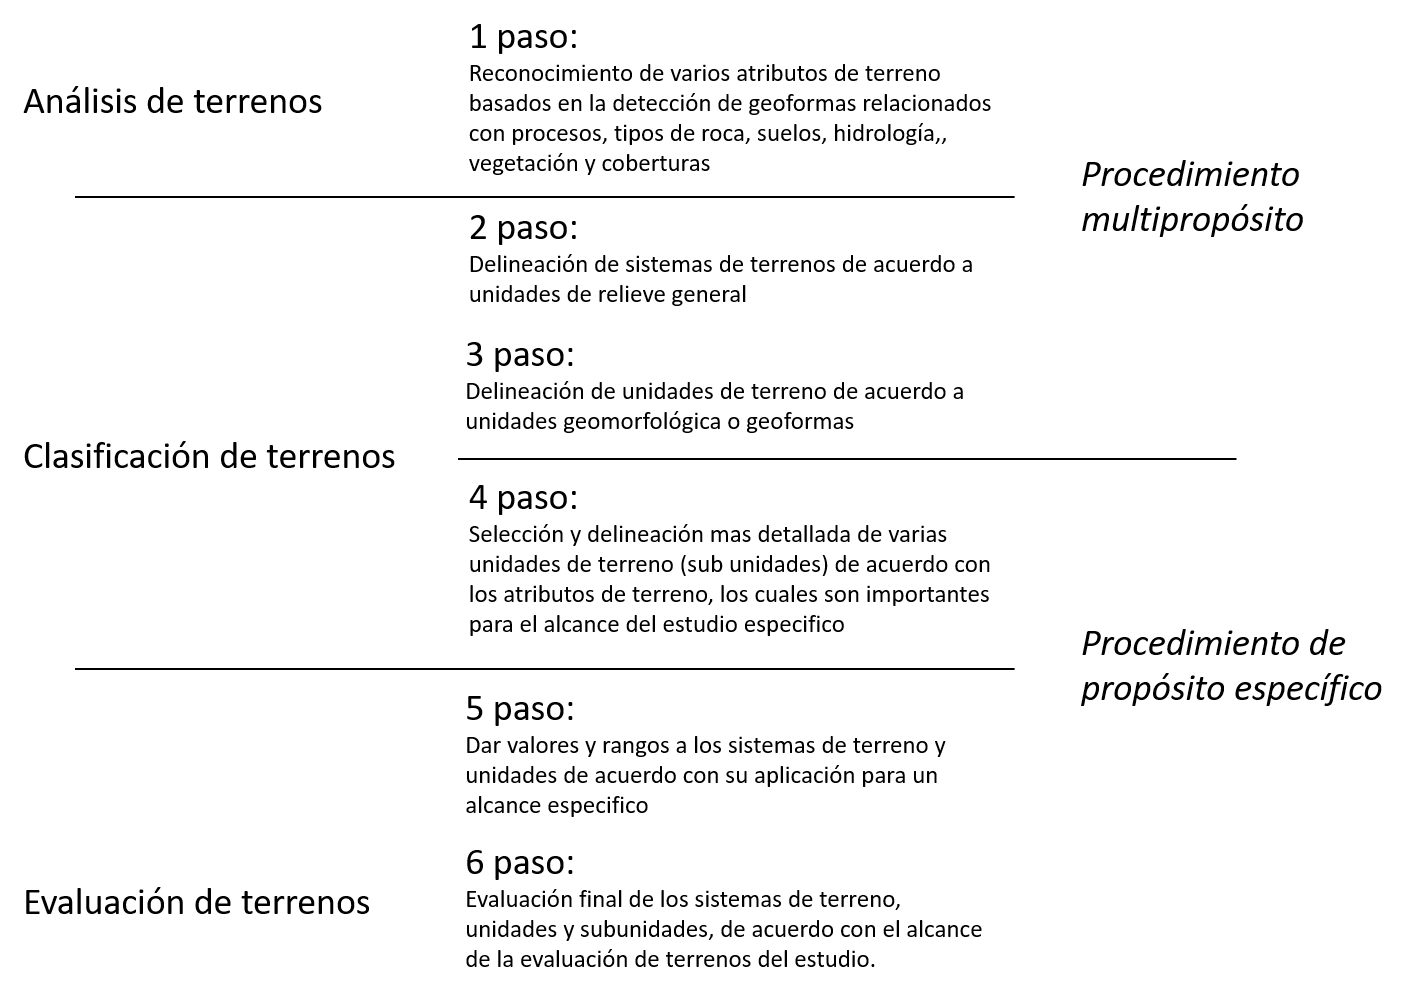
\includegraphics[scale=0.42]{metocarto}
\end{center}
\tiny{Fuente: van Zuidam (1985)}
\end{frame}
%%%%%%%%%%%%%%%%%%%%%%%%%%%%%%%%%%%%%%%%%%%%%%%%%%%%%%%%%%%%%%%%%%%%%%%%%
\begin{frame}
\frametitle{Metodologia ITC}
\begin{center}
   	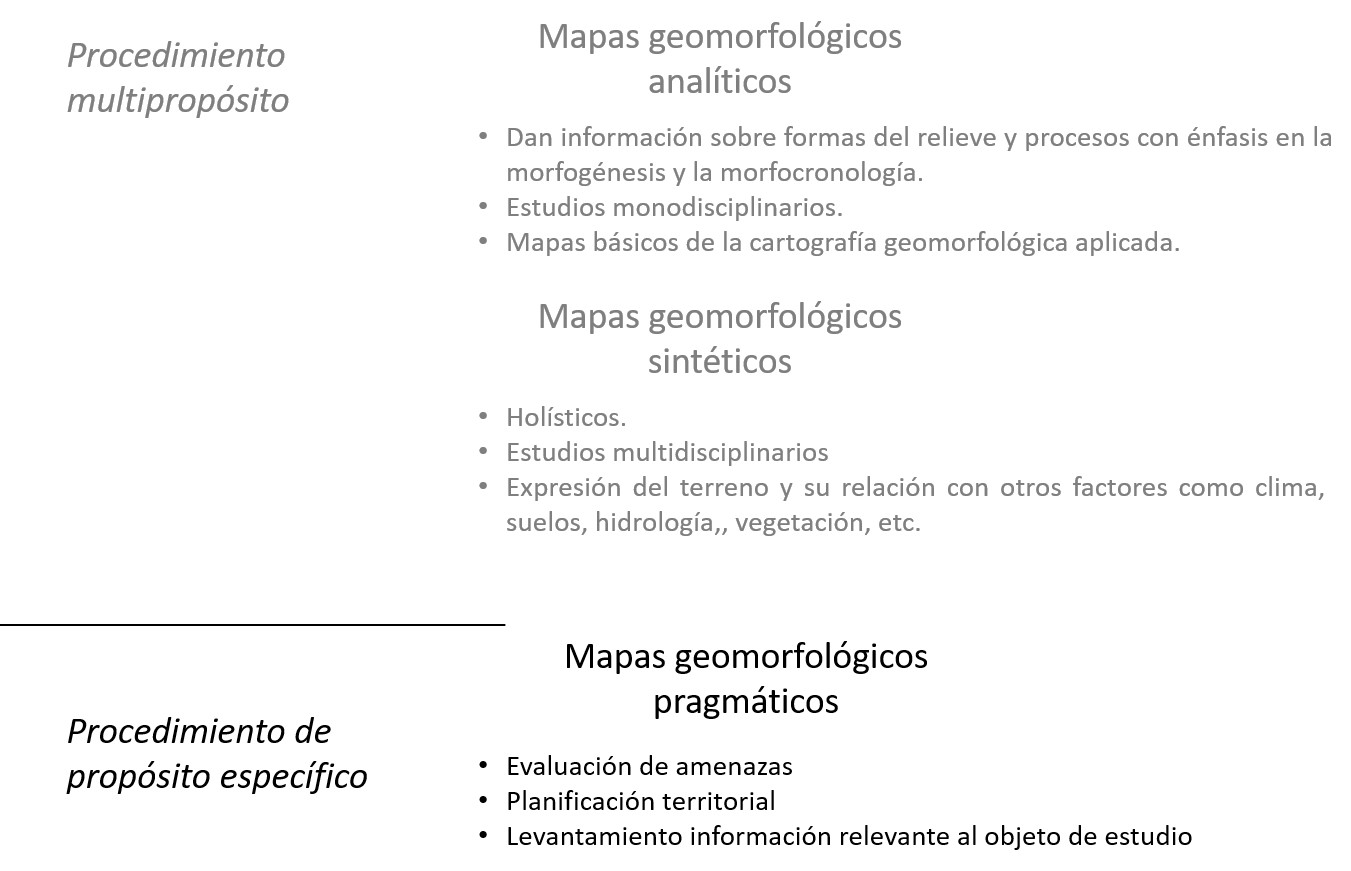
\includegraphics[scale=0.44]{metocarto1}
\end{center}
\tiny{Fuente: van Zuidam (1985)}
\end{frame}
%%%%%%%%%%%%%%%%%%%%%%%%%%%%%%%%%%%%%%%%%%%%%%%%%%%%%%%%%%%%%%%%%%%%%%%%%
\begin{frame}
\frametitle{Análisis Heurístico}
\framesubtitle{Cartografía Geomorfológica Directa}
\begin{center}
   	\includegraphics[scale=0.44]{heuristico_geomor}
\end{center}
\tiny{Fuente: van Zuidam (1985)}
\end{frame}
%%%%%%%%%%%%%%%%%%%%%%%%%%%%%%%%%%%%%%%%%%%%%%%%%%%%%%%%%%%%%%%%%%%%%%%%%
\begin{frame}
\frametitle{Cartografía Geomorfológica Directa}
\begin{center}
   	\includegraphics[scale=0.44]{mapageomorfologico3}
\end{center}
\tiny{Fuente: Barredo et al. (2000)}
\end{frame}
%%%%%%%%%%%%%%%%%%%%%%%%%%%%%%%%%%%%%%%%%%%%%%%%%%%%%%%%%%%%%%%%%%%%%%%%%
\begin{frame}
\frametitle{Cartografía Geomorfológica Directa}
\framesubtitle{Zonificación de amenaza}
\begin{center}
   	\includegraphics[scale=0.44]{amenaza}
\end{center}
\tiny{Fuente: Barredo et al. (2000)}
\end{frame}
%%%%%%%%%%%%%%%%%%%%%%%%%%%%%%%%%%%%%%%%%%%%%%%%%%%%%%%%%%%%%%%%%%%%%%%%%
\begin{frame}
\frametitle{Zonificación geológico-geotécnica}
\framesubtitle{Unidad Morfológico-Geológica de Comportamiento Geomecánico Independiente (UGI)}
\small{Combinación de criterios morfológicos, litológicos y estructurales que permitan delimitar una zona cuya estabilidad no depende del comportamiento de las zonas vecinas y complementariamente el caso inverso. Inicialmente se puede aceptar que los límites de esta unidad básica son los cambios definitivos de pendientes (cuchillas, valles aluviales, cañones profundos, terrenos planos, etc,); sin embargo las unidades litológicas presentes, sus propiedades geomecánicas y las estructuras geológicas pueden llevar a una ampliación o a una reducción de la unidad básica geomorfológicamente delimitada.}
\begin{center}
   	\includegraphics[scale=0.42]{mapageotecnico}
\end{center}
\tiny{Fuente: China (1998)}
\end{frame}
%%%%%%%%%%%%%%%%%%%%%%%%%%%%%%%%%%%%%%%%%%%%%%%%%%%%%%%%%%%%%%%%%%%%%%%%%
\begin{frame}
\frametitle{Zonificación geológico-geotécnica}
\justifying
\begin{itemize}
\small{
\item \textbf{Subzonas tipo A – Estable independiente}: su estabilidad es de alto grado pues sus condiciones naturales son favorables. Posiblemente llegaría a depender del manejo mismo que se le dé al terreno.
\item \textbf{Subzonas tipo B – Estable dependiente}: su estabilidad depende de factores externos, los cuales se deben corregir. También de factores internos que implican un manejo determinado del terreno y cierto tipo de obras civiles que granticen el no deterioro de esta estabilidad natural inicial.
\item \textbf{Subzonas tipo C – Inestable recuperable}: la estabilidad de estos terrenos es critica o presenta inestabilidad manifiesta; sin embargo, con algunos correctivos específicos se puede mejorar la estabilidad, y en consecuencia, adelantar ciertas obras civiles en si interior.
\item \textbf{Subzonas tipo D – Inestable no recuperable}: terrenos con inestabilidad manifiesta cuya recuperación no es posible o demasiado costosa comparada con las inversiones y tipo de obras proyectadas.
\item \textbf{Subzonas tipo E – Estable no utilizable}: terrenos estables pero restringidos por condiciones urbanísticas u otras como estar ubicadas en vegas potenciales de inundación o cerca de frentes libres de taludes desprotegidos.
\item \textbf{Subzonas tipo F – Inestables no utilizables}: terrenos inestables y restringidos por condiciones como las mencionadas para la zubzona anterior.
}
\end{itemize}
\end{frame}
%%%%%%%%%%%%%%%%%%%%%%%%%%%%%%%%%%%%%%%%%%%%%%%%%%%%%%%%%%%%%%%%%%%%%%%%%
\begin{frame}
\frametitle{Zonificación geológico-geotécnica}
\begin{center}
   	\includegraphics[scale=0.44]{mapageotecnico1}
\end{center}
\tiny{Fuente: Barredo et al. (2000)}
\end{frame}
%%%%%%%%%%%%%%%%%%%%%%%%%%%%%%%%%%%%%%%%%%%%%%%%%%%%%%%%%%%%%%%%%%%%%%%%%
\begin{frame}
\frametitle{Red de drenajes}
\begin{center}
   	\includegraphics[scale=0.44]{trellis}
\end{center}
\end{frame}
%%%%%%%%%%%%%%%%%%%%%%%%%%%%%%%%%%%%%%%%%%%%%%%%%%%%%%%%%%%%%%%%%%%%%%%%%
\begin{frame}
\frametitle{Geomorfología fluvial}
\begin{center}
   	\includegraphics[scale=0.44]{meandros2}
\end{center}
\end{frame}
%%%%%%%%%%%%%%%%%%%%%%%%%%%%%%%%%%%%%%%%%%%%%%%%%%%%%%%%%%%%%%%%%%%%%%%%%
\begin{frame}
\frametitle{Geomorfología fluvial}
\begin{center}
   	\includegraphics[scale=0.44]{geofluvial}
\end{center}
\end{frame}
%%%%%%%%%%%%%%%%%%%%%%%%%%%%%%%%%%%%%%%%%%%%%%%%%%%%%%%%%%%%%%%%%%%%%%%%%
\begin{frame}
\frametitle{Trabajo en grupo}
\begin{center}
   	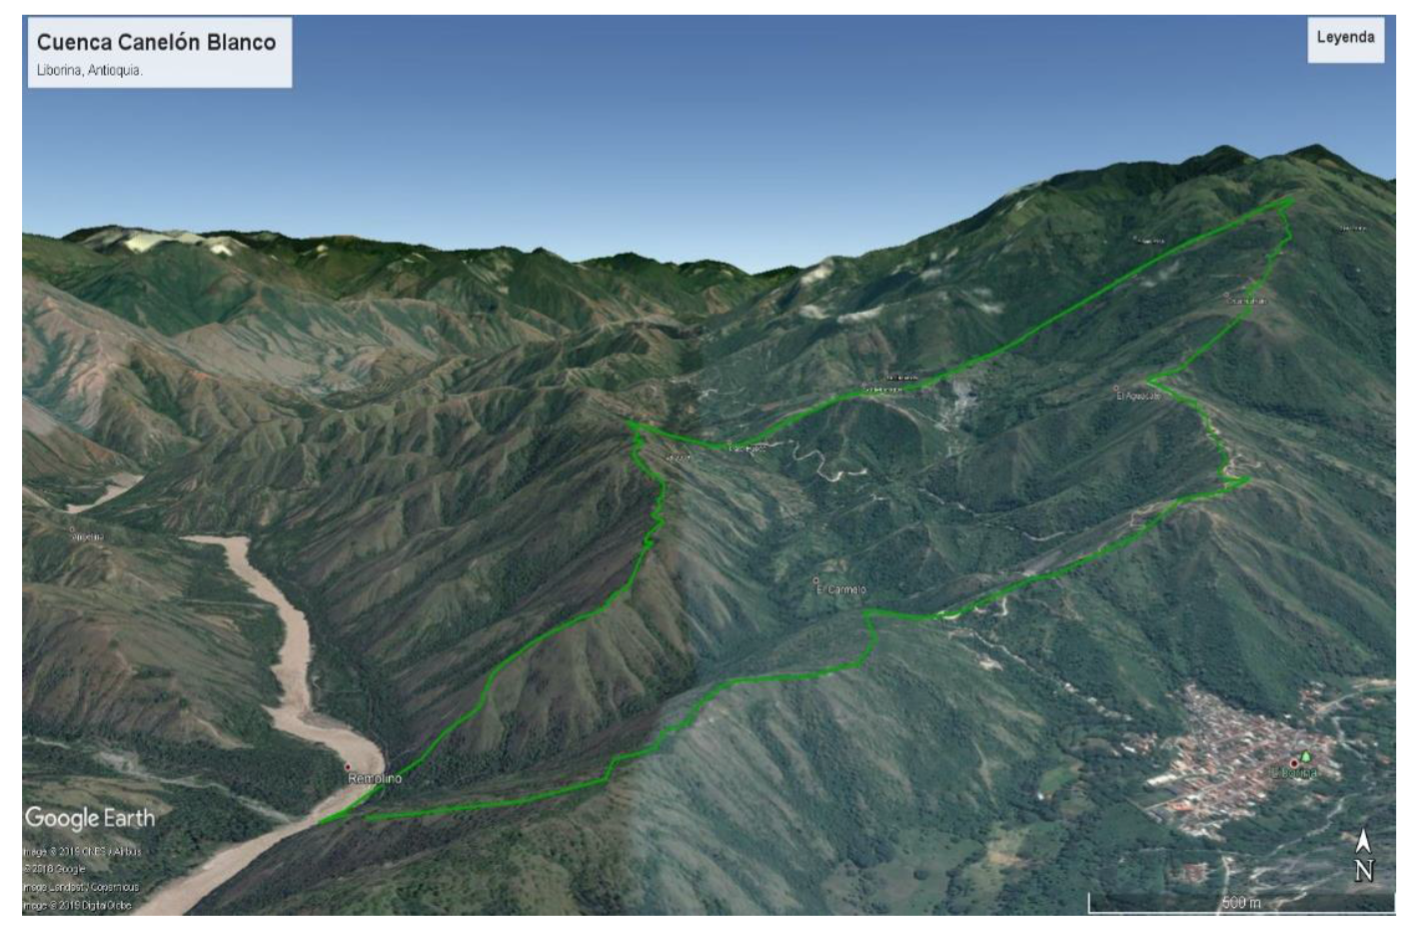
\includegraphics[scale=0.44]{cuencatrabajo}
\end{center}
\end{frame}
%%%%%%%%%%%%%%%%%%%%%%%%%%%%%%%%%%%%%%%%%%%%%%%%%%%%%%%%%%%%%%%%%%%%%%%%%
\end{document}